%
%	Theorieteil
%

\pagebreak
\section{mTLS Exploration}

\onehalfspacing

\subsection{Sample Voting Application}

To evaluate mTLS and service mesh, we will use a simple application, the \href{https://github.com/dockersamples/example-voting-app}{example-voting-app} from the official \href{https://github.com/dockersamples}{Docker Samples}; it's a simple distributed application running across multiple Docker containers, and we will follow Sathish Kumar's excellent post about deploying it on Kubernetes using slightly modified deployment files.\footnote{See \textit{Kumar, S. (2021)}: Deploying a sample microservices app with Kubernetes. \cite{votingApp}}

The application has the following architecture:\footnote{See \textit{Kumar, S. (2021)}: Ibid. \cite{votingApp}}

\begin{figure}[H]
\centering
\caption {Application Architecture}
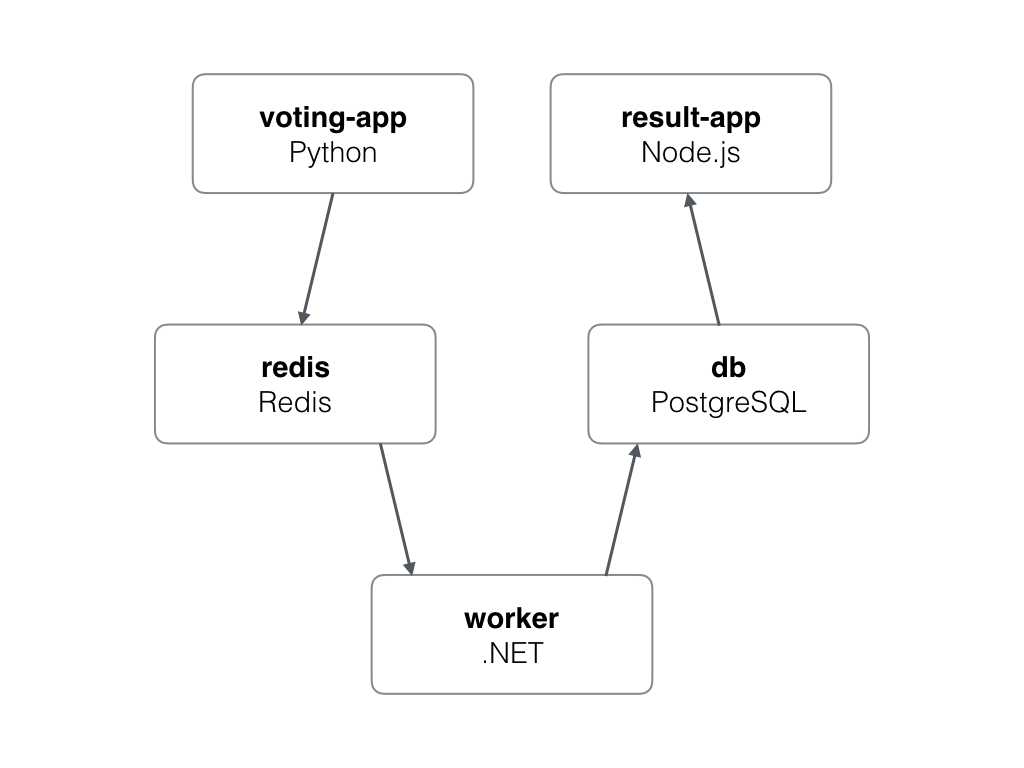
\includegraphics[width=\linewidth]{images/architecture.png}
\label{fig:votingApp}
\end{figure}

It consists of the following components:

\begin{itemize}
    \item A front-end web app
    \item A Redis database collecting new votes
    \item A worker consuming votes and storing them
    \item A Postgres database
    \item A Node.js web app showing the results\footnote{See \textit{Docker (2024)}: Example Voting App. \cite{votingGithub}}
\end{itemize}

After deploying the application, these components will run inside the Kubernetes cluster, each as an individual pod:

\begin{figure}[H]
\centering
\caption {Voting Application Components}
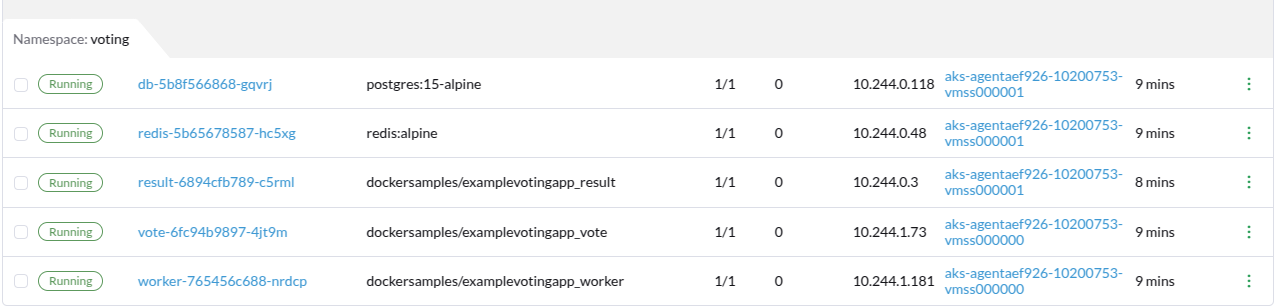
\includegraphics[width=\linewidth]{images/voting-pods.png}
\label{fig:votingPods}
\end{figure}

The YAML files used for the application deployment are on the paper's \href{https://github.com/chfrank-cgn/Hausarbeit-DF/tree/main/voting}{Github}.

Using Rancher's security component Neuvector, we can examine the network connections of the application components:

\begin{figure}[H]
\centering
\caption {Voting Application Connections}
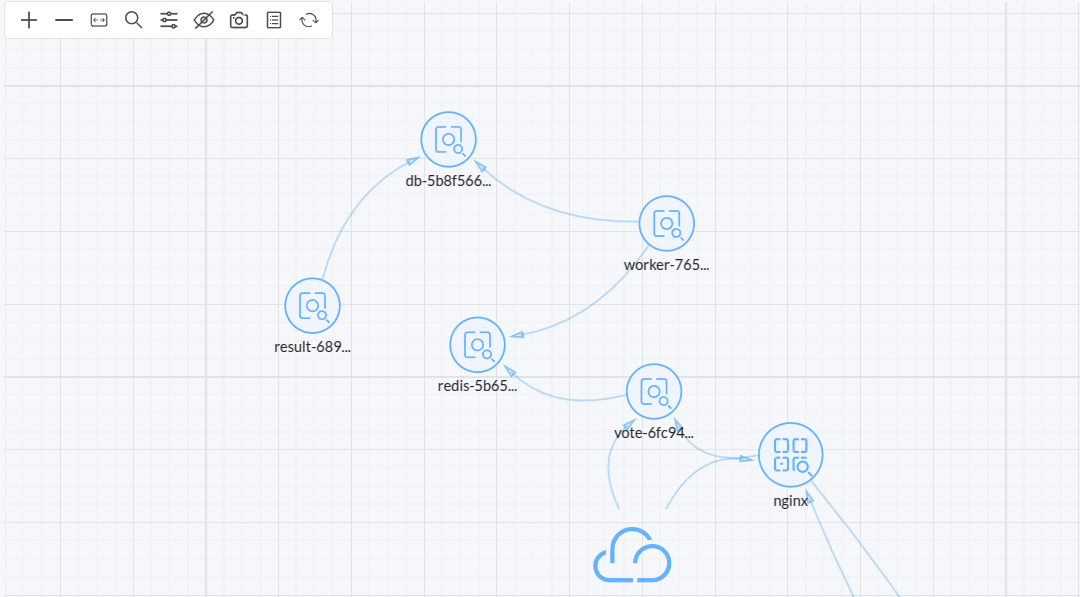
\includegraphics[width=\linewidth]{images/voting-map.png}
\label{fig:votingMap}
\end{figure}

\begin{itemize}
    \item Outside communication will reach the vote front-end, initially through the AKS ingress controller
    \item The vote component will connect to the Redis in-memory database
    \item The worker component will connect to both the Redis and the Postgres database
    \item The result component will read from the Postgres database
\end{itemize}

The arrows indicate the direction in which the connections were established. Without any installed service mesh, all connections are unencrypted. The observed communication relationships match the application documentation.

\subsection{Linkerd}

To install Linkerd edge-25.1.2, we follow the instructions provided by SUSE\footnote{See \textit{Dayley, B. (2021)}: End-to-end Encryption with Linkerd. \cite{installLinkerd}} and the reference documentation provided by Linkerd.\footnote{See \textit{Linkerd (2025)}: Getting Started. \cite{gettingStarted}}

After installation, the Linkerd control plane adds four pods to the running cluster.

\begin{figure}[H]
\centering
\caption {Linkerd Components}
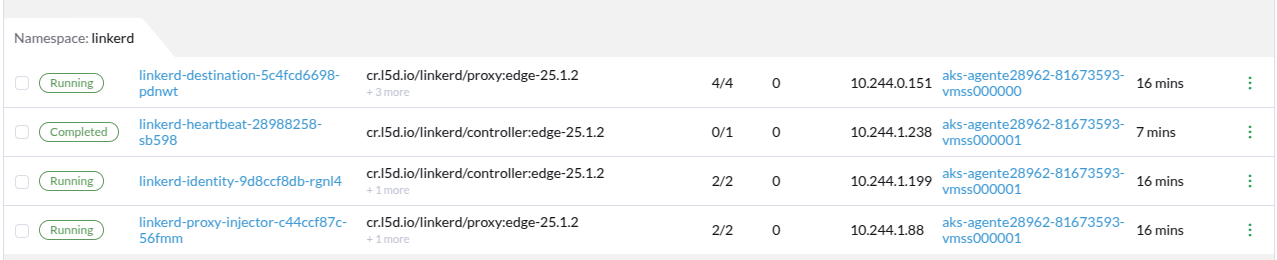
\includegraphics[width=\linewidth]{images/linkerd-pods.png}
\label{fig:linkerdPods}
\end{figure}

Using the Linkerd CLI, we inject our voting application with the service mesh information.

\begin{verbatim}
    kubectl get -n voting deploy -o yaml \
    | linkerd inject - \
    | kubectl apply -f -
\end{verbatim}

Linkerd will then add a proxy sidecar to each application pod to enable the service mesh functionality and encrypt the application traffic.

\begin{figure}[H]
\centering
\caption {Linkerd Application Connections}
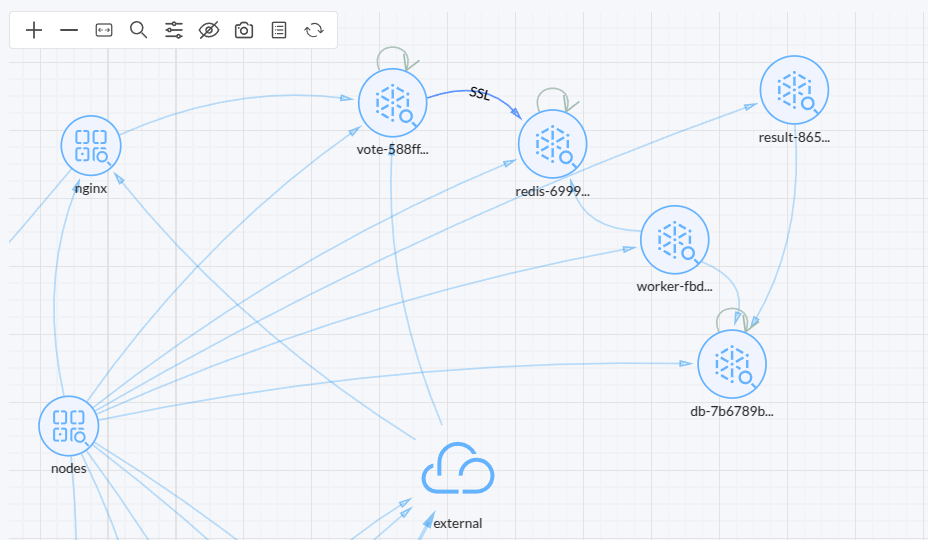
\includegraphics[width=\linewidth]{images/linkerd-map.png}
\label{fig:linkerdMap}
\end{figure}

The network diagram shows that the traffic between the vote and the Redis component is now encrypted with TLS.

In the default installation, only the traffic is encrypted. Linkerd offers the capability to encrypt the traffic and add authentication and authorization using Linkerd policies.\footnote{See \textit{Linkerd (2025)}: Restricting Access To Services. \cite{restrictingAccess}}

This paper will only look at mTLS encryption and leave authentication for future investigations.

\subsection{Istio}

To install Istio 1.24.1, we again follow the instructions provided by SUSE.\footnote{See \textit{Rancher Labs (2025)}: Enable Istio in the Cluster. \cite{enableIstio}} As with Linkerd, enabling mTLS for applications in the mesh will be automatic.\footnote{See \textit{Istio (2025)}: mTLS in Istio. \cite{istioMtls}} 

Istio requires the Rancher Monitoring application or any other Prometheus deployment to be installed on the cluster first.\footnote{See \textit{Rancher Labs (2025)}: Enable Monitoring. \cite{enableMonitoring}}

After installation, the Istio adds three pods to the running cluster.

\begin{figure}[H]
\centering
\caption {Istio Components}
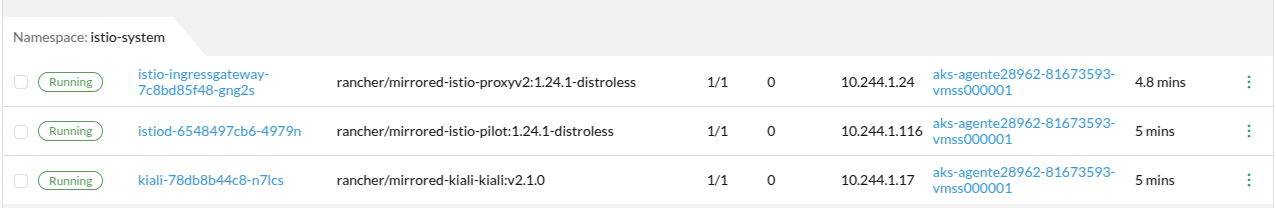
\includegraphics[width=\linewidth]{images/istio-pods.png}
\label{fig:istioPods}
\end{figure}

For Istio, we use the auto-inject feature on the application namespace to inject our voting application with the service mesh information.

\begin{verbatim}
    "kubernetes_namespace": {
      "name": "voting",
      "labels": {
        "field.cattle.io/projectId": "p-g89q2",
        "istio-injection": "enabled",
        "kubernetes.io/metadata.name": "voting"
      }
    }
\end{verbatim}

Istio will then add a proxy sidecar to each application pod during deployment in this namespace to enable the service mesh functionality and encrypt the application traffic.

\begin{figure}[H]
\centering
\caption {Istio Application Connections}
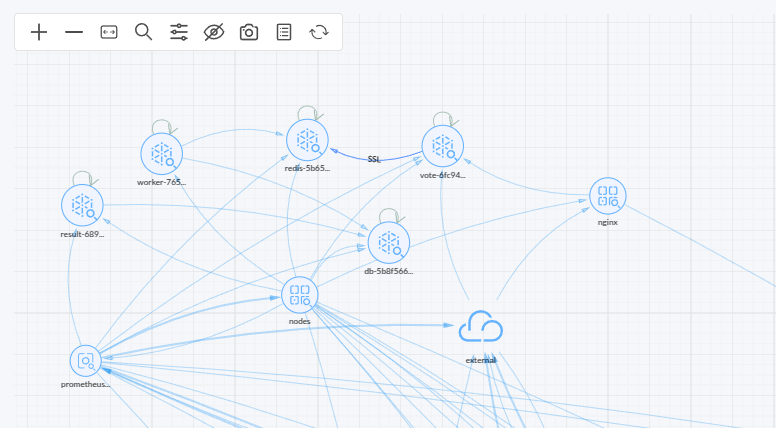
\includegraphics[width=\linewidth]{images/istio-map.png}
\label{fig:IstioMap}
\end{figure}

As with Linkerd, the network diagram now shows that the traffic between the vote and the Redis component is encrypted with TLS. There are a number of additional connections due to the requirement for metrics collection with Prometheus.

Istio also offers the option to authenticate connections.
